
\section{Introduction}
\subsection{Background \& Motivation}
Two-wheeled vehicles are generally more agile, allowing easier navigation through tight spaces, making them ideal for congested environments. Their lighter weight and compact size facilitate easier handling while also enhancing energy efficiency. In addition, they are typically less expensive to purchase and maintain, increasing accessibility for a wider range of users.
A good base model to build such robot is \href{https://www.elegoo.com/products/elegoo-tumbller-self-balancing-robot-car}{ELEGOO Tumbler} (shown in Fig. 
\ref{fig:tumbler}), which provided nearly all the hardware required as a DIY kit.

\begin{figure}[h]
	\centering
	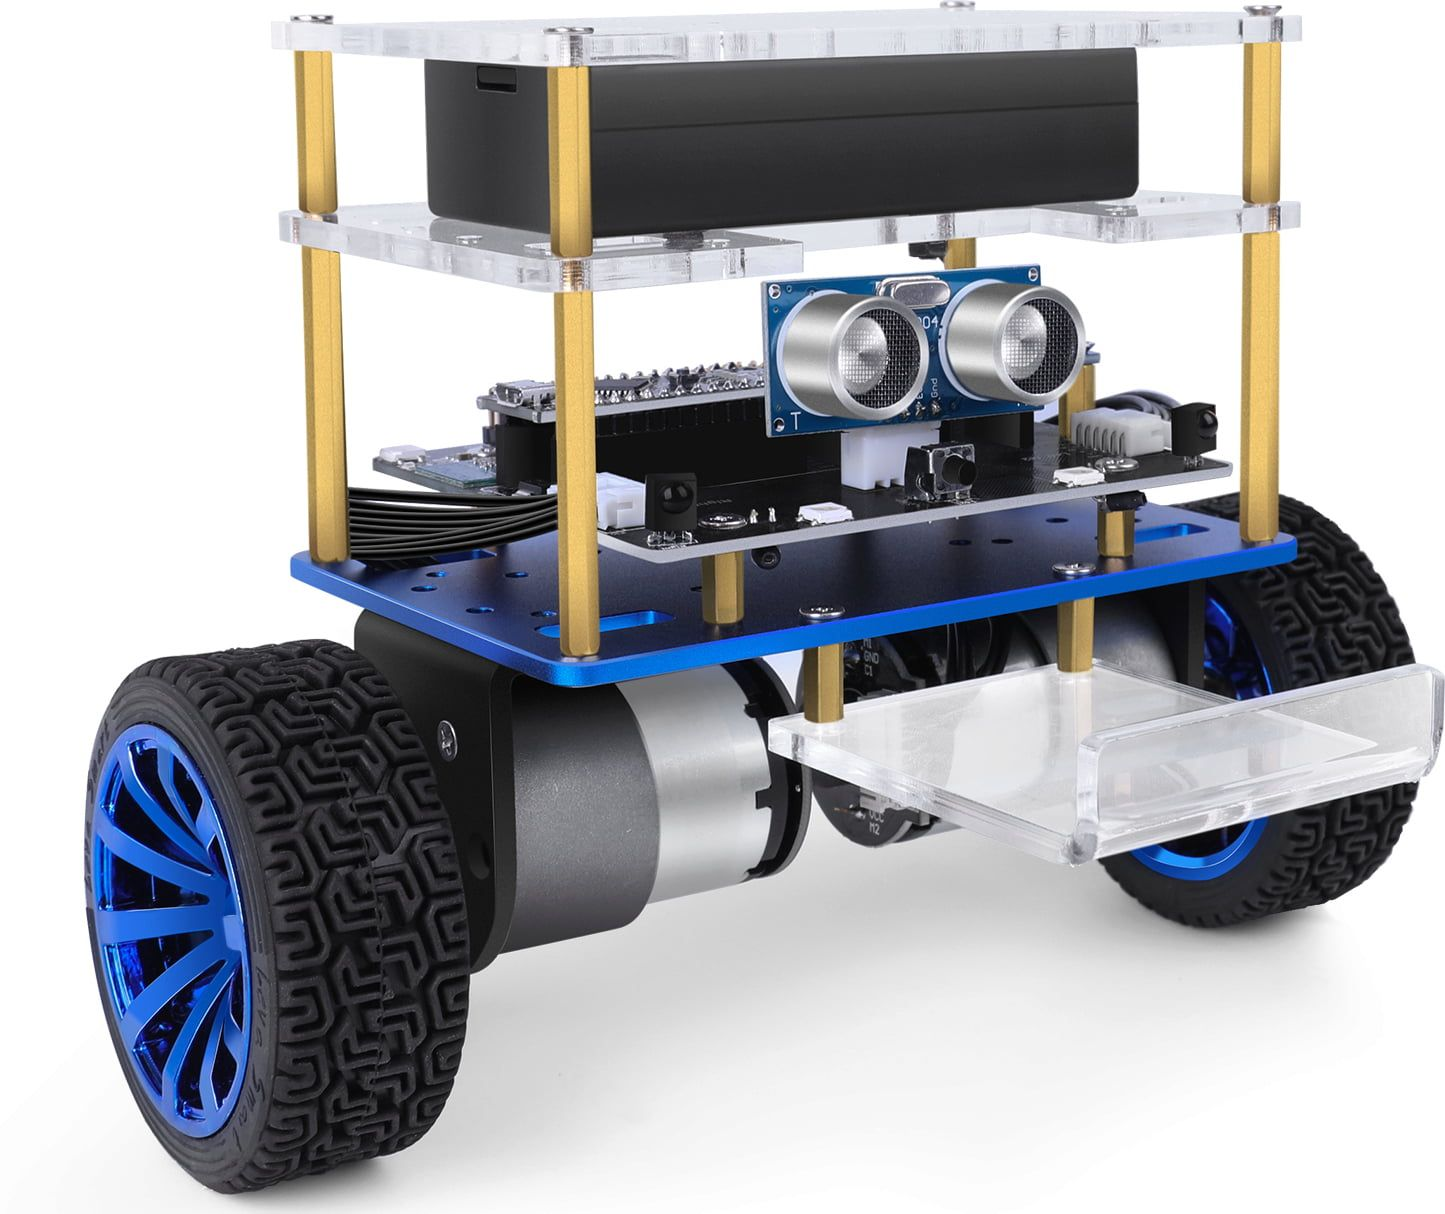
\includegraphics[height=6cm]{assets/tumbller.jpg}
	\caption{\label{fig:tumbler} ELEGOO Tumbler which was used for this project \cite{tumbller}.}
\end{figure}

\subsection{Project Objectives}
The primary objectives of this project are as follows:
\begin{itemize}
	\item To design and implement a two-wheeled self-balancing robot capable of maintaining stability using sensor feedback and control algorithms.
	\item To develop a cascaded PID control system for real-time balance and motion control, ensuring robustness and responsiveness.
	\item To integrate an MPU6050 inertial measurement unit (IMU) for accurate state estimation, utilizing sensor fusion techniques such as a Kalman filter.
	\item To enable remote monitoring and control of the robot, enhancing its versatility for various applications.
	\item To document the design, implementation, and tuning processes, providing a comprehensive resource for future development and replication.
\end{itemize}


\section{Literature Review}
Two-wheeled self-balancing robots have been widely studied as a variant of the classic inverted pendulum problem, requiring advanced control strategies to maintain stability. Various approaches, including Proportional-Integral-Derivative (PID) control \cite{matlab_inverted_pendulum}, Linear Quadratic Regulator (LQR)~\cite{10193276} have been explored to achieve robust balancing and motion control.

Xu and Duan~\cite{1174486} demonstrated that the Linear Quadratic Regulator (LQR) controller outperforms the pole-placement controller in both simulation and real-time control scenarios.

Kalman filtering has been extensively used for sensor fusion in such systems, particularly for integrating accelerometer and gyroscope data to obtain accurate state estimates. Studies have demonstrated that complementary and extended Kalman filters significantly improve stability and noise rejection in sensor-driven control systems.

Recent advancements in autonomous navigation for self-balancing robots have incorporated Simultaneous Localization and Mapping (SLAM) techniques, LiDAR-based obstacle detection, and machine learning-based adaptive control methods \cite{Tsai_Chih_2008} \cite{Ranasinghe_Vidanapathirana_2019}. These improvements enable real-time path planning and environmental interaction, making self-balancing robots more suitable for real-world applications such as personal mobility, surveillance, and industrial automation.

This project builds upon these existing methodologies by implementing a Kalman filter for sensor fusion and employing PID-based control to achieve stable balancing and maneuverability. Future work aims to integrate more advanced control and navigation techniques for enhanced autonomy and performance.

\subsection{Scope of Work}
The scope of this project encompasses the following key areas:
\begin{itemize}
	\item \textbf{Hardware Integration:} Assembling and configuring the ELEGOO Tumbler platform, including the MPU6050 IMU, motor drivers, and encoders.
	\item \textbf{Software Development:} Implementing firmware for the Arduino Nano microcontroller using PlatformIO, focusing on sensor data acquisition, control algorithms, and communication protocols.
	\item \textbf{Control System Design:} Designing and tuning a cascaded PID control loop for pitch, yaw, and position control, ensuring stable and precise operation.
	\item \textbf{Sensor Fusion:} Utilizing a Kalman filter to fuse data from the IMU, improving the accuracy of state estimation and control.
	\item \textbf{Testing and Validation:} Conducting extensive testing to evaluate the robot's performance under various conditions, followed by iterative refinement of the control parameters.
	\item \textbf{Documentation and Open-Source Contribution:} Providing detailed documentation, including schematics, code, and tuning guidelines, and making the project available on a \href{https://github.com/haris-mujeeb/Self-Balancing-Robot}{GitHub repository} for open-source collaboration \cite{opensource}.
\end{itemize}

\begin{figure}[h]
	\centering
	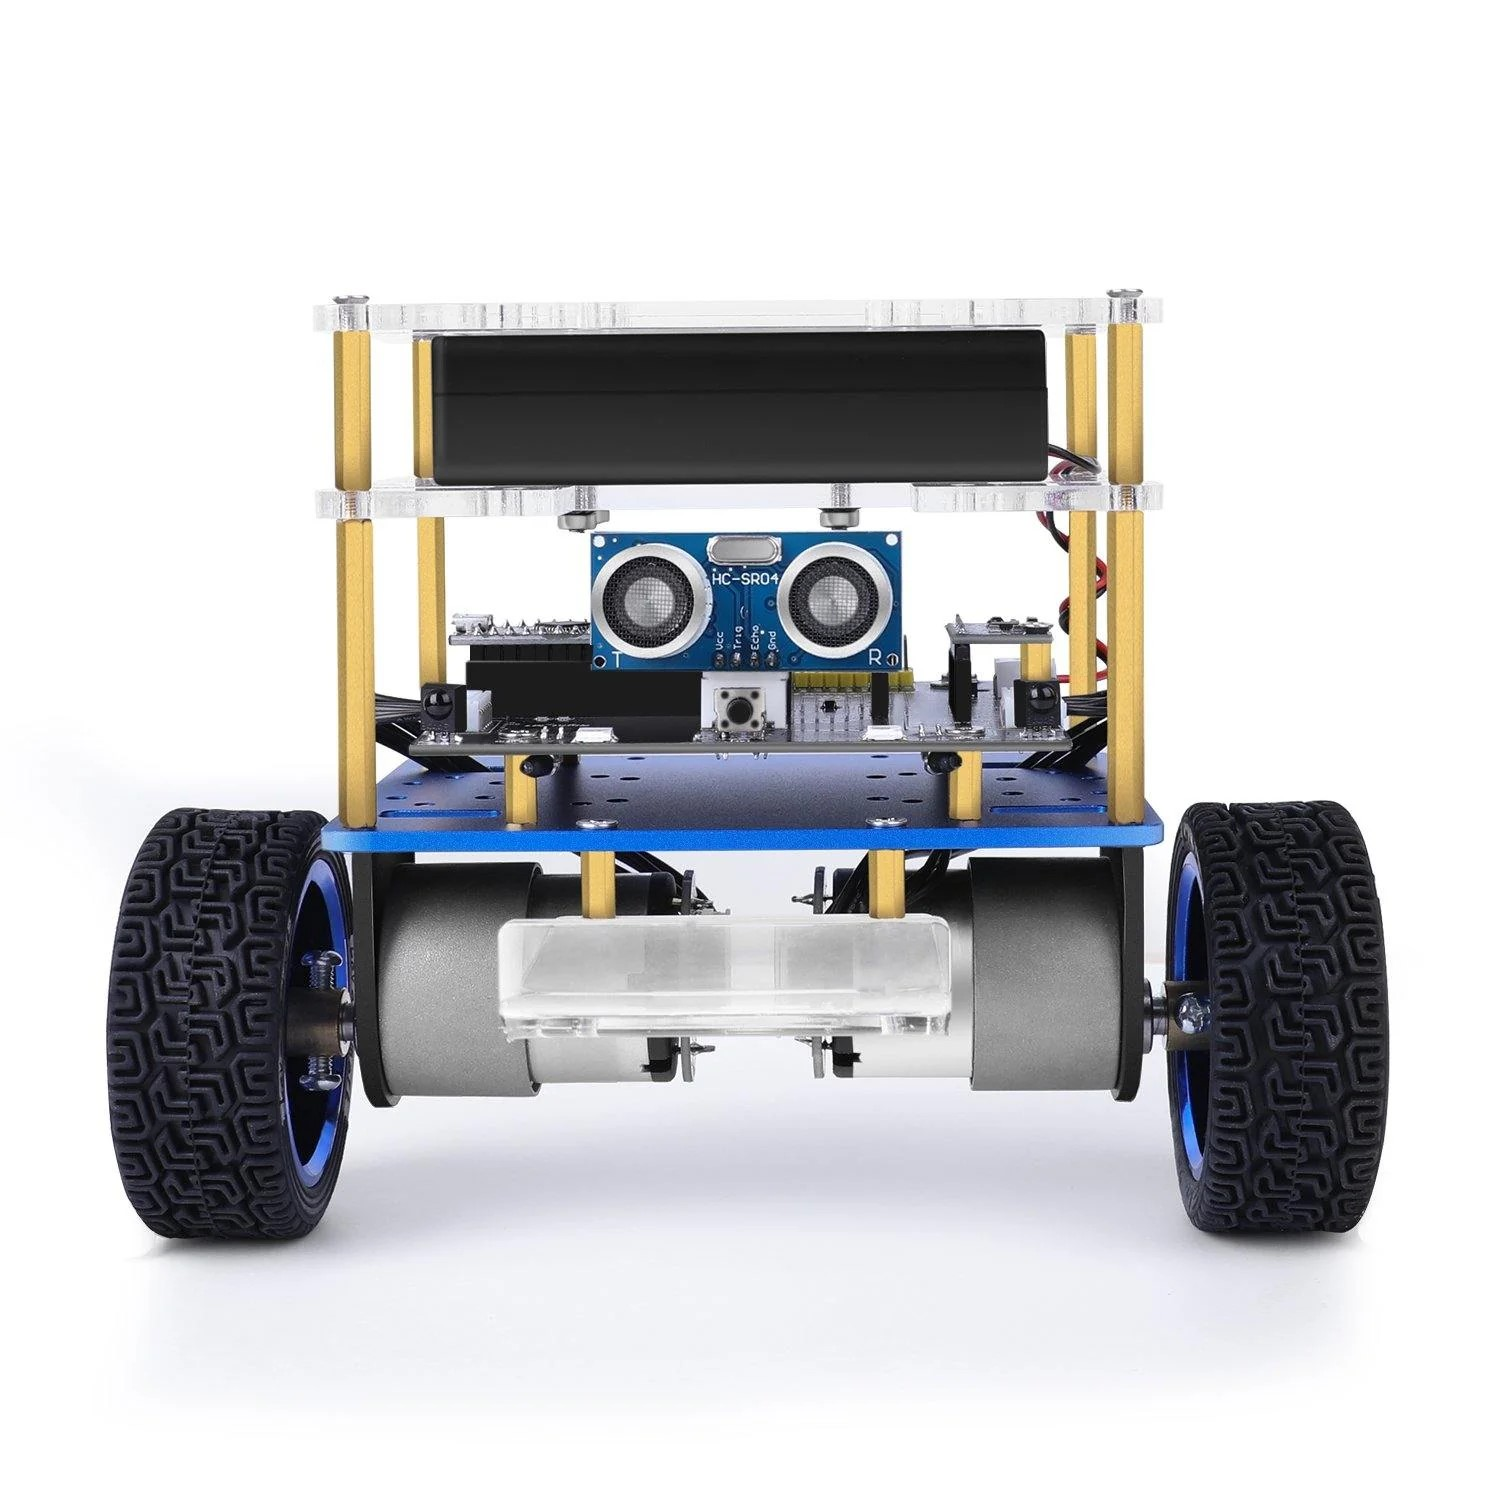
\includegraphics[height=6cm]{assets/tumbller2.jpg}
	\caption{\label{fig:tumbler2} ELEGOO Tumbler \cite{tumbller}.}
\end{figure}